\newpage
\section{Лекция 8}
\subsection{Сингулярный и Спектральный радиусы}
Повторим несколько утверждений из предыдущих лекций.
\begin{itemize}
    \item В каждом векторном пространстве $V(\mathbb{R},~\mathbb{C})$ есть норма $\nu(\bar x)\geqslant 0$ такая, что:\begin{enumerate}
        \item $\nu(\bar x) > 0$, $\bar x \neq \bar 0$, $\nu(\bar 0) = \bar 0$
        \item $\nu(\alpha \bar x) = |\alpha|\nu(\bar x)$
        \item $\nu(\bar x + \bar y) \leq \nu(\bar x) + \nu(\bar y)$ для $\forall x, y \in V, \forall \alpha$
    \end{enumerate}
    \item Норма Гёльдера: \begin{center}
        $|\bar x|_1=|x_1|+\cdots +|x_n|$\\
        $|\bar x|_2=\sqrt{|x_1|^2+\cdots +|x_n|^2}$\\
        $|\bar x|_{\infty}=\underset{i=1,\cdots,n}{max}|x_i|$ \end{center}
    \item В конечномерном пространстве все нормы эквивалентны.
    \item Свойства матричной нормы $M\in M_n$: 
    \begin{enumerate}
        \item $||AB||\leqslant ||A||\cdot ||B||$
        \item Матричная норма $||\cdot||$ на $M_n$ согласована с векторной нормой $|\cdot|$ на $\mathbb{C}^n$, если $$|Ax|\leqslant ||A||\cdot |x|$$
        \item Матричная норма сохраняет единицу, если $||E||=1$.
    \end{enumerate}
    \item Норма Фробениуса: $||A||_F=\sqrt{\sum\limits_{i,j}|a_{ij}|^2}$. Она удовлетворяет свойствам 1, 2 для $|\cdot|_{1,~2,~\infty}$, но не удовлетворяет свойству 3.
    \item $||\cdot||_{\star}$ --- индуцированная матричная норма, если верно $$||A||_{\star}=\underset{\bar x \neq \bar 0}{max} \cfrac{|Ax|_{\star}}{|x|_{\star}}=\bigg( y=\cfrac{\bar x}{|\bar x|_{\star}} \bigg)=\underset{|y|_{\star}=1}{max}|Ay|_{\star}$$
\end{itemize}

\textbf{Пример 1.}\\
Найти $y$ для матрицы $A$ \[A=\begin{pmatrix}
1 & 2\\
3 & 4
\end{pmatrix}\]
\begin{center}
    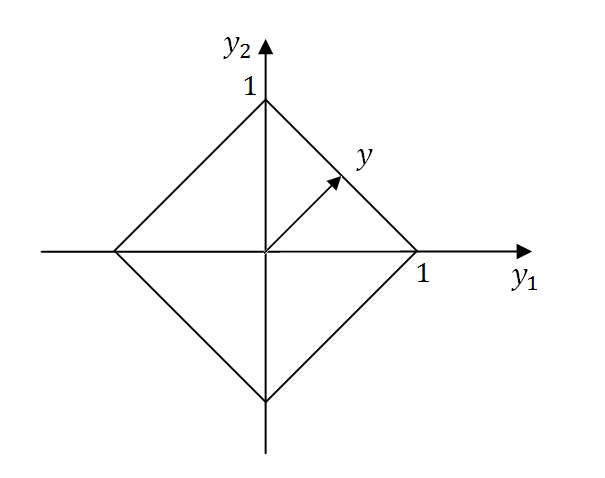
\includegraphics[scale=0.6]{l8_1.png}\end{center}
\[y=\begin{pmatrix}
y_1\\
y_2
\end{pmatrix}\]
$$||A||_1=max|A \bar y|=\underset{|y_1|+|y_2|=1}{max}|y_1+2y_2|+|3y_1+4y_2|$$
Максимум получим при $y_1=0$ и $y_2=1$: $||A||_1=2+4=6$.
\[y=\begin{pmatrix}
0\\
1
\end{pmatrix}\]
\begin{definition}
    \textbf{Сингулярным радиусом} матрицы $A$ называется её максимальное сингулярное значение: $\sigma(A) = \sigma_1$.
\end{definition}
\begin{theorem}
    $||A||_2=\sigma(A)$
\end{theorem}
\begin{proof}
    Вспомним, что такое сингулярное разложение матрицы (SVD): $$A=V\Sigma U^*$$
    $V, ~U$ --- унитарные матрицы ($U^*=U^{-1}$). Найдём сингулярное разложение для матрицы $AA^*$.
    \[\Sigma=\begin{pmatrix}
    \sigma_1 & \cdots & 0\\
    \vdots & \ddots & \vdots\\
    0 & \cdots & \sigma_n
    \end{pmatrix}\]
    Тогда $$(A^*A)^*=A^*A=U\Sigma V^* V \Sigma U^*=U\Sigma^2 U^*$$
    \[\Sigma^2=\begin{pmatrix}
    \sigma_1^2 & \cdots & 0\\
    \vdots & \ddots & \vdots\\
    0 & \cdots & \sigma_n^2
    \end{pmatrix}\]
    $\sigma_1 \geqslant \sigma_2 \geqslant \cdots \geqslant \sigma_n \geqslant 0$ --- сингулярные значения матрицы.\\
    Аналогично $$AA^*=V\Sigma^2 V^*$$
    Здесь $U^1,\cdots,U^n$ --- ортонормированный базис из собственных векторов матрицы $A^*A$, а $V^1,\cdots,V^n$ --- ортонормированный базис из собственных векторов матрицы $AA^*$. $U^i$ и $V^i$ --- правые и левые сингулярные векторы соответственно.
    
    Теперь перейдём к доказательству.
    $$||A||_2=\underset{|x|_2=1}{max}|Ax|_2=\underset{|x|_2=1}{max} \sqrt{(Ax, Ax)}=\underset{|x|_2=1}{max}\sqrt{(Ax)^*Ax}=\underset{|x|_2=1}{max}\sqrt{x^*A^*Ax}$$
    $$A^*A\overset{\alpha\to U}{\rightarrow}\Sigma^2$$
    $$x=\sum\limits_i \alpha_i U_i,~\sum\limits_i|\alpha_i|^2=1$$
    $$xx^*=\sum\limits_i \alpha_i U_i U_i^* \alpha_i=\sum\limits_i \alpha_i U_i U_i^{-1} \alpha_i=\sum\limits_i|\alpha_i|^2$$
    \begin{center}
        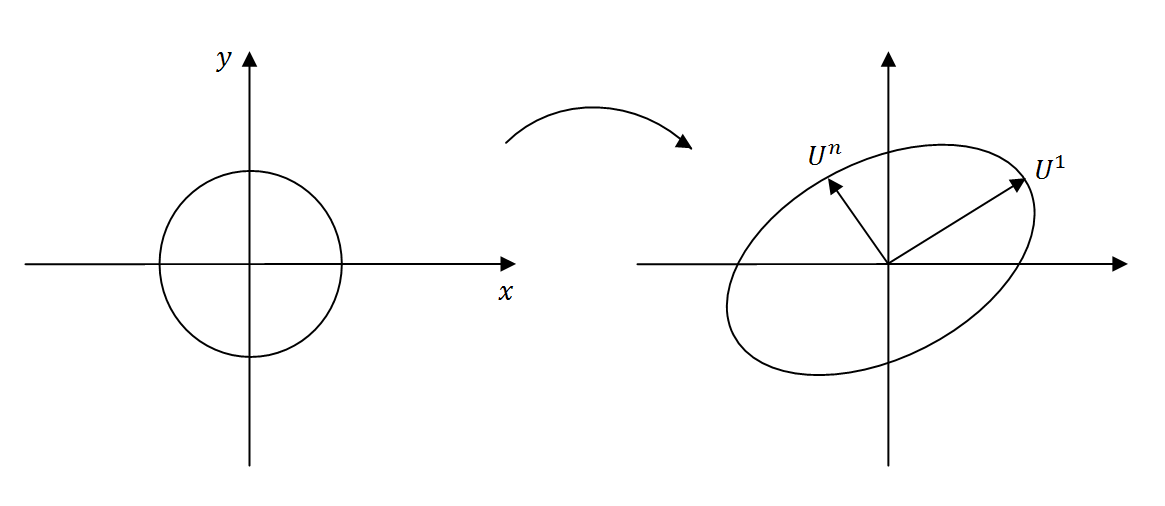
\includegraphics[scale=0.6]{l8_2.png}\end{center}
    Подставим в $||A||_2$:\begin{center}
        $||A||_2=\underset{|x|_2=1}{max}\sqrt{x^*A^*Ax}=$(в базисе $U$)$=\underset{|x|_2=1}{max}\sqrt{x\Sigma^2 x^*}=\underset{\alpha:~\sum\limits_i |\alpha_i|^2=1}{max}\sqrt{\sum\limits_i \sigma_i^2 |\alpha_i|^2}=\underset{\alpha:~\sum\limits_i |\alpha_i|^2=1}{max}\sqrt{\sigma_1^2|\alpha_1|^2+\cdots+\sigma_n^2|\alpha_n|^2} \leqslant \underset{\alpha:~\sum\limits_i |\alpha_i|^2=1}{max} \sqrt{\sigma_1^2(|\alpha_1|^2+\cdots+|\alpha_n|^2)}=\sigma_1$\end{center}
\end{proof}

\begin{definition}
    \textbf{Матричная норма Фробениуса}:
    $$||A||_F=\sqrt{\sum\limits_{i,j}|a_{ij}|^2}=\sqrt{tr(A^*A)}$$
\end{definition}
\begin{statement}
    $||A||_F = \sqrt{\sigma_1^2+\sigma_2^2+\cdots+\sigma_n^2}$.
\end{statement}
\begin{proof}
    \[A^*A=\begin{pmatrix}
    \bar a_{11} & \cdots & \bar a_{n1}\\
    * & * & *\\
    * & * & *
    \end{pmatrix} \cdot \begin{pmatrix}
    a_{11} & * & *\\
    \vdots & * & *\\
    a_{n1} & * & *
    \end{pmatrix} = \begin{pmatrix}
    \bar a_{11} a_{11}+\cdots+\bar a_{n1} a_{n1} & * & *\\
    * & * & *\\
    * & * & *
    \end{pmatrix}=\] \[=\begin{pmatrix}
    |a_{11}|^2+\cdots +|a_{n1}|^2 & * & *\\
    * & * & *\\
    * & * & *
    \end{pmatrix}\]
    Получим $\sqrt{tr(A^*A)}=\sqrt{\sigma_1^2+\sigma_2^2+\cdots+\sigma_n^2}$.
\end{proof}


\[A=\begin{pmatrix}
1 & 2\\
0 & 3\\
\end{pmatrix}\]
$||A||=1$ ?\begin{center}
    $||A||_F=\sqrt{1^2+2^2+3^2}=\sqrt{14}$\\
    $||A||_F \geqslant ||A||_2 \geqslant \cfrac{1}{\sqrt{n}}||A||_F=\sqrt{7}$\\
    $||A||_1=\underset{j}{max}\sum\limits_i|a_{ij}|=max\{1,~5\}=5$\\
    $||A||_{\infty}=\underset{i}{max}\sum\limits_j|a_{ij}|=max\{3,~3\}=3$\end{center}
\begin{definition}
    \textbf{Спектральный радиус} матрицы $A$ -- это модуль её наибольшего собственного значения. $\rho(A)=|\lambda_{max}(A)|=\underset{i}{max}|\lambda_i|$
\end{definition}
\begin{theorem}
    Если матричная норма $||\cdot||$ согласована с некоторой векторной нормой, то $$||A|| \geqslant \rho(A)$$
\end{theorem} 
\begin{proof}
    $ Av=\lambda v,~v\neq 0$ --- для собственного значения существует собственный вектор.\\
    Из определения согласованности векторной нормы: $|Av|\leqslant ||A||\cdot|v|$.
    С другой стороны, $|Av|=|\lambda v|=|\lambda||v|$. Получим, что $|\lambda|\leqslant ||A||$, то есть, норма не меньше, чем $\lambda.$
\end{proof}
\begin{consequence}
        В частности $$\sigma(A)\geqslant \rho(A)$$
\end{consequence}
\begin{center}
    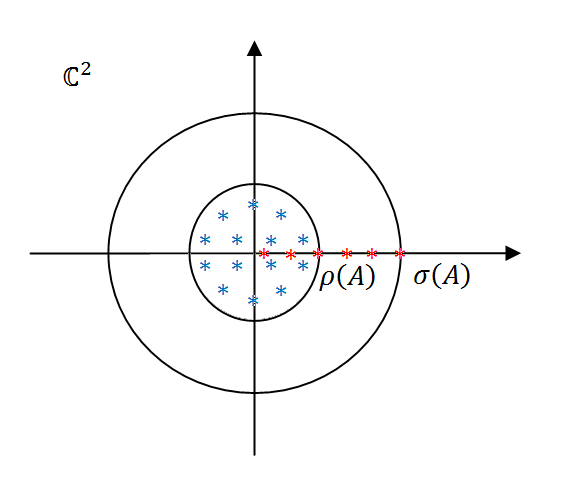
\includegraphics[scale=0.6]{l8_3.png}\end{center}
Здесь $\sigma_i(A)$ --- сингулярные собственные значения, а $\rho(A)~(\lambda_i(A))$ --- собственные значения.

\begin{statement}
    Для любой матрицы $A$ и $\forall~ \varepsilon>0$ существует матричная норма $||\cdot ||$, согласованная с некоторой векторной нормой $|\cdot|$, и такая, что $$||A||\leqslant \rho(A) + \varepsilon$$
    С помощью $\varepsilon$ можно добиться равенства.
\end{statement}

\subsection{Приближённое разложение меньшего ранга}
Разложение матрицы $A_{n \times n}=A_{n \times r} \cdot A_{r \times
    n}$, $A$ ранга $r$.\\
\textbf{Как получить приближенное разложение матрицы?}\\
$A\approx X$, $X$ ранга $r$, $X$ --- ?\\
\textbf{Задача:} найти $X$ ранга $\leqslant r$ такое, что $$||X-A||\to min$$\\
\textbf{Ответ:} для матричных норм $||\cdot||_2,~||\cdot||_F$ (и любой ортогонально инвариантной) $$A=V\Sigma U^*$$
\[\Sigma=\begin{pmatrix}
\sigma_1 & \cdots & 0\\
\vdots & \ddots & \vdots\\
0 & \cdots & \sigma_n
\end{pmatrix}\]
\[\Sigma_r=\begin{pmatrix}
\sigma_1 & \cdots & 0  & \cdots & 0\\
\vdots & \ddots & \vdots & \vdots & \vdots\\
0 & \cdots & \sigma_r &  \vdots & \vdots\\
\vdots & \cdots & \cdots & \ddots & \vdots\\
0 & \cdots & \cdots & \cdots & 0\\
\end{pmatrix}\]
$$X=A_r=V\Sigma_r U^*$$
Для $||A||=||A||_2=\sigma(A)$.
\begin{proof}[Корректность]
$U^1,\cdots, U^n$ --- правый сингулярный базис.
Пусть $\bar w \in <U^1,\cdots,U^{r+1}> \cap~ Ker X$, где $Ker X \geqslant n-r$, а $X$ ранга $\leqslant r$, $|w|=1$.\\
Так как $|Mx|\leqslant ||M||,~|x|=1$, тогда \begin{center}
    $(||X-A||_2)^2 \geqslant(|(X-A)w|_2)^2=|Xw-Aw|^2=|Aw|^2=$ (в базисе $U$) =
\end{center}
\[=\Bigg| V\begin{pmatrix}
\sigma_1 & \cdots & 0  & \cdots & 0\\
\vdots & \ddots & \vdots & \vdots & \vdots\\
0 & \cdots & \sigma_{r+1} &  \vdots & \vdots\\
\vdots & \cdots & \cdots & \ddots & \vdots\\
0 & \cdots & \cdots & \cdots & 0\\
\end{pmatrix} \begin{pmatrix}
w_1\\
\vdots\\
w_{r+1}\\
\vdots\\
0\\
\end{pmatrix}\Bigg|^2 =\Bigg|V \begin{pmatrix}
\sigma_1 w_1\\
\vdots\\
\sigma_{r+1} w_{r+1}\\
\vdots\\
0\\
\end{pmatrix} \Bigg|^2 =\Bigg| \begin{pmatrix}
\sigma_1 w_1\\
\vdots\\
\sigma_{r+1} w_{r+1}\\
\vdots\\
0\\
\end{pmatrix} \Bigg|^2=\]$$=\sigma_1^2|w_1|^2+\cdots+\sigma_{r+1}^2|w_{r+1}|^2 \geqslant \sigma_{r+1}^2(|w_1|^2+\cdots+|w_{r+1}|^2)=\sigma_{r+1}^2|w|=\sigma_{r+1}^2$$ для любой матрицы $X$, где 
\[||A_r-A||_2=||V(\Sigma-\Sigma_r)U^*||_2=||\Sigma-\Sigma_r||_2 = \Bigg| \Bigg|\begin{pmatrix}
0 & \cdots & 0  & \cdots & 0\\
\vdots & \ddots & \vdots & \vdots & \vdots\\
0 & \cdots & \sigma_{r+1} &  \vdots & \vdots\\
\vdots & \cdots & \cdots & \ddots & \vdots\\
0 & \cdots & \cdots & \cdots & \sigma_n\\
\end{pmatrix}\Bigg|\Bigg|_2=\sigma_{r+1}\]
Достигается для $r$, значит она оптимальна (меньше нет). Для евклидовой нормы это лучшее приближение.
\end{proof}
\textbf{Пример 2.}\\
Найти наилучшее приближение $A_1$ ранга 1 для матрицы $A$ в норме $||\cdot||_2$ и найти $||A-A_1||_2$, где
\[A = \begin{pmatrix}
6 & 0 & 6\\
0 & 12 & 6\\
6 & 6 & 9
\end{pmatrix}\]
Так как матрица $A$ симметричная, можно не находить $A^*A$. Найдем сразу собственное значение и собственный вектор.
\begin{center}
    $det(A-\lambda E)=0$\\
    $\lambda_1=18,~\lambda_2=9,~\lambda_3=0$\end{center}
\[\Sigma = \begin{pmatrix}
18 & 0 & 0\\
0 & 9 & 0\\
0 & 0 & 0
\end{pmatrix}\]
Хотим построить сингулярное разложение $A=V\Sigma U^*$. Если $A^*=A$, то $V=U$.\\
После решения СЛАУ $(A-\lambda_i E)x=0$ из $\lambda_i$ получим $v_i$.
\[V=U= \begin{pmatrix} [r]
\cfrac{1}{3} & \cfrac{2}{3} & -\cfrac{2}{3}\\
\cfrac{2}{3} & -\cfrac{2}{3} & -\cfrac{1}{3}\\
\cfrac{2}{3} & \cfrac{1}{3} & \cfrac{2}{3}
\end{pmatrix}\]
\[\Sigma_1 = \begin{pmatrix}
18 & 0 & 0\\
0 & 0 & 0\\
0 & 0 & 0
\end{pmatrix}\]
\[X=A_1 = V\Sigma_r U^*=\begin{pmatrix}
2 & 4 & 4\\
4 & 8 & 8\\
4 & 8 & 8
\end{pmatrix}\]
Ранг матрицы $A_1$ равен $1$, $||A-A_1||_2=9$ (наибольший из остальных $\sigma$).\\ \\
\subsection{Домашнее задание 8}
\begin{enumerate}
    \item
    Найти наилучшее приближение ранга 2 по фробениусовой норме для матрицы 
    \[B = \begin{pmatrix}
    6 & 0 & 6\\
    0 & 12 & 6\\
    6 & 6 & 9
    \end{pmatrix}\]
    
    \item Найти наилучшее приближение $B_1$ ранга 1 для матрицы $B$ в норме $||\cdot||_2$ и найти $||B-B_1||_2$, где
    \[B = \begin{pmatrix}
    6 & 30 & -21\\
    17 & 10 & -22\\
    \end{pmatrix}\]
    
    \item Доказать утверждение из лекции: для любой матрицы $A$ и $\forall~ \varepsilon>0$ существует матричная норма $||\cdot ||$, согласованная с некоторой векторной нормой $|\cdot|$ и такая, что $$||A||\leqslant \rho(A) + \varepsilon .$$
\end{enumerate}